\documentclass[letterpaper, 10 pt, conference]{ieeeconf}

\IEEEoverridecommandlockouts
\overrideIEEEmargins

\usepackage{times}
\usepackage{mathptmx}
\usepackage{amsmath}
\usepackage{amsfonts}
\usepackage{amssymb}
\usepackage{graphicx}
\usepackage{multicol}
\usepackage[utf8]{inputenc}
\usepackage{array}
\usepackage{lipsum}
\graphicspath{{images/}}
\usepackage{parskip}
\usepackage{indentfirst}
\usepackage{courier}
\usepackage{wrapfig}
\usepackage{caption}
\usepackage[left=1.5in, right=1in, top = 1in, bottom = 1in]{geometry}
\usepackage{float}
\usepackage[ruled]{algorithm}
\usepackage{algpseudocode}
\usepackage{graphicx}
\usepackage{url}
\usepackage{cite}
\usepackage{rotating}
\usepackage{subcaption}

\parindent 10pt
\parskip 2ex

\begin{document}

\begin{center}
	\huge Critical Encounters
	
	\large Hunter Figueroa, Zachary Painter, Jacob Spigle, \& David Akridge
	
	\large Department of Electrical Engineering and Computer Science, University of Central Florida, Orlando, Florida, 32816-2450
\end{center}

\

\begin{abstract}
	This paper presents, in detail, the design process for creating our website, Critical Encounters. Critical Encounters is a web-based platform designed to streamline the process
	for players of the d20 Game System to create, test, and play through their own
	creations, including encounters and monsters, in order to play more effectively
	in a live setting. Users are able to publicly post their created encounters for
	others to play through and review, and utilize our stress-tester for more in-depth
	statistics about their creation.
\end{abstract}

\small \textbf{\textit{Index Terms}--- Creativity, crowdsourcing, digital simulation, internet, user centered design.}

\

\section{Introduction}

Role-playing games are games where players act as their characters. Usually
in person, around a table, and controlled by the players speaking their actions
in turn. This might not always be done by speaking in-character, but rather by
following this basic structure:
\begin{enumerate}
	\item The GM describes the environment.
	\item The players describe what they want to do.
	\item The GM narrates the results of the characters actions.
\end{enumerate}
\par
There are countless possible character, monster, and scenario possibilities when
constructing a tabletop role-playing campaign, however, it is hard and sometimes
impossible to sift through them all and find the perfect encounter. Not only that,
but once you commit to a game or role-playing decision you are forced to see it
through to completion in order to retain the game’s continuity. Players get one
chance to design their character at the very start of a session, and once they do,
that character’s path cannot be meaningfully changed. Spending so much time
working on a character, and then coming to the first session to find out that they
are severely unprepared for the tasks they are presented can be harrowing. On the
other side, the GM spends so much time outside of the game to prepare a story
and encounters that challenge the Players, so when that GM accidentally wipes
out the entire team of Player Characters (PCs) in one unbalanced encounter, or
if the PCs simply walk through a fight that was meant to challenge them for the
remainder of the session, the GM feels they have failed the PCs in presenting a
good game. \par
This project presents a service that can be used by both GMs and players to
test out their characters, encounters, team builds, or boss fights in a simulated
environment. This allows users to figure out just how well their creation holds
up to the requirements that they have set for themselves, and perfect them to
ensure the most enjoyable experience in a live game encounter.
This project seeks to develop a service that allows a user to create an encounter
that follows the rules of the d20 Game System. The creator streamlines the refining
process by easily being able to simulate the encounter. By allowing the player or
GM to import their character’s/monsters’ statistics and equipment, they then
can play against an automated opponent or opponents using that creation. Encounters have the ability to be rapidly simulated over and over to display
statistics about the encounter the help improve the encounter. To further enhance
a user’s ability to test and refine encounters and PCs, users are able to upload
and share their encounters to their public space where others can try their own
creations’ skills in that creator’s setting.

\section{Overview of Requirements}

This project was pitched by the group in the beginning of the Senior Design I semester, and as such, did not have a formal sponsor throughout the development process. The scale of the project and thus the requirements that the website Critical Encounters would achieve was based on the aspects that we felt were important to have completed by the end of the Senior Design II term. We knew that by the end of the formal project deadline we would have the following completed:
\begin{enumerate}
	\item Website hosted where it could be accessible from any device.
	\item Encounter Creator Tools present so users could invent their own combat centric encounters inside Critical Encounters, and the ability to host them on the website in their own space, their ``Arena''.
	\item Combatant Creation, where users could customize their own PC or monster.
	\item Battlefield where users could simulate a full encounter using either their own created encounter or those hosted by other users on the website against a DM or PC A.I. simulation, while using their own created PC or monster against the encounter creator's combatants present in the encounter.
	\item After completing an encounter on the website, users would be able to view statistics about the combat and review for their own usage. Users would also be encouraged to leave a review of the played encounter so the creator would receive feedback as well.
	\item The ability for users to save/load ongoing combat encounters.
	\item Users would be able to search for Arenas \& Encounters, while also being able to filter those results by tags, ratings, and time since the encounter was uploaded.
	\item An Encounter Diagnostic Tool would be implemented to allow users to run the system through a large amount of testing all at once, and receive statistics aggregated from those tests in order to better adjust their encounter for live gaming. 
\end{enumerate}

\section{High Level Block Diagram}
	\begin{figure}[H]
	\centering
	\centerline{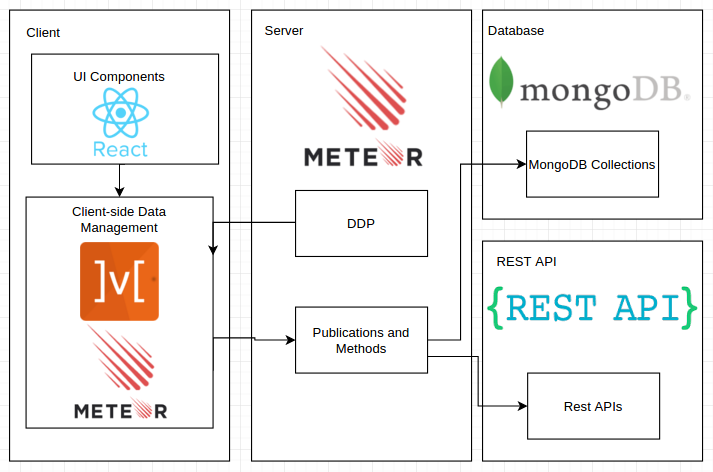
\includegraphics[scale=.3]{high_level_block_diagram}}
	\caption{High Level Block Diagram}
	\label{fig: High Level Block Diagram }
	\end{figure}

We have implemented a Client-Server Design structure that is commonly used
with web applications such as Critical Encounters. There are three areas of production
in this high-level design: Server, Database/Rest API and Client-Side. The UI
components are developed in REACT and control the the MVC system.
Data management on the client-side are managed by MobX and Meteor, the
latter of which serves as the point of contact with the server-side of the app.
The server is developed in Meteor, and is responsible for contacting
the database, developed in MongoDB and performing REST API commands when
necessary.
The relationship between client and server is a pseudo model-view-controller
architecture. Where REACT acts as the as application’s view and Meteor/-
MobX acts as both the controller and the model. Meteor with MobX automatically manages the data flow, client state, and client rendering. \par
Meteor uses an ORM/MERN, Object-relational mapping / MongoDB
- Express - React, stack design pattern. It focuses on model driven development,
in which the models are shared between the server and the client. This
is seen most clearly seen in the MiniMongo database cache that is accessible by
the font-end front end and can asynchronously update the MongoDb REST API
is implemented automatically which translates to automatic database updates.

\section{Conclusions}

Tabletop games bring people together in a world where physical interaction is
often lost in lieu of digital communication. This project aims to supplement these
interactions by making them more accessible to newer players, as well as help
experienced players spend less time on pre-game preparation. In-game encounters
require large amounts of time to plan, setup, and implement, so by enhancing
this process and giving the GM the ability to perfect an encounter beforehand the
whole process becomes more enjoyable for anyone playing the game.
\par Critical Encounters has the potential to broaden the audience of an already quickly
expanding pastime to younger players and DM’s. Concepts in the realm of tabletop
games are very easily understood by a younger audience, as their imagination and
creativity can run free in such games. However, the threshold of understanding
for the many rules and balances may prove a bit overzealous for this audience.
Having a service that improves accessibility to newer players  also bleeds
into improving accessibility for younger players as well. Additionally, users who
do not have a group to play with may find and form groups with other users with
whom they have played and shared content with.

\section*{APPENDIX}

\listoffigures

\begin{thebibliography}{99}

\bibitem{c1} 

\end{thebibliography}




\end{document}
